\documentclass[a4paper,12pt]{article}
\usepackage[utf8x]{inputenc}
\usepackage{ucs}
\usepackage[T1]{fontenc}
\linespread{1.2}
\usepackage{amsmath,amssymb,amsthm,amsfonts,ulem}
\usepackage{courier, fourier}
\usepackage{clrscode3e}
\usepackage{mdwlist}
\setcounter{secnumdepth}{0}
\setcounter{tocdepth}{3}
\usepackage{todonotes}
\usepackage{hyperref}

\usepackage{subcaption}
\usepackage{float}
\usepackage{mdwlist}
\usepackage{wrapfig}
\usepackage{caption}
\newcommand{\graphicc}[4]{\begin{figure}[H] \centering
            \includegraphics[width={#1\textwidth}, keepaspectratio=true]{{#2}}
            \caption{{#3}} \label{#4} \end{figure}}

\title{Examn notes for Advanced Algorithms and Datastructures 2014}
\author{Martin Jørgensen}
\date{\today}

\begin{document}

\maketitle

\tableofcontents
\pagebreak

\section{Dispositions}
\subsection{Max-Flow}
\begin{enumerate}
  \item (Define a Flow Network)
    \begin{itemize*}
      \item (Capacity Constraint)
      \item (Flow Conservation)
    \end{itemize*}
  \item Define a Max Flow
  \item (How to have multible source/sink networks)
  \item (Introduce Residual Networks)
  \item (Introduce Augmenting Paths)
  \item Cuts - In particular the min cut max flow
  \item Introduce Ford-Fulkerson / Edmonds-Karp
\end{enumerate}
\newpage

\subsection{Fibonacci Heaps}
\begin{enumerate}
  \item Mergeable heaps
  \item Structure
  \item Operations
    \begin{itemize*}
      \item Make-Heap
      \item Insert
      \item ExtractMin
      \item Union/Merge
      \item DecreaseKey
      \item Delete
    \end{itemize*}
\end{enumerate}
\todo[inline]{Wrwite something about $D(n)$ since it's used for all the proofs.}
\newpage

\subsection{NP-Completeness}
\begin{enumerate}
  \item Polynomial time vs Superpolynomial time
  \item P-Class problems
  \item NP-Class problems
  \item Decisions vs Optimization problems
  \item Reductions and verifiability/certificates
  \item P vs NP vs NPC
\end{enumerate}
\newpage

\subsection{Randomized Algorithms}
\begin{enumerate}
  \item Las-Vegas vs. Monte Carlo Algorithms
  \item Decision Monte Carlo, one sided vs. two sided error.
  \item Bounding Runningtimes
  \item Markov \& Chebyshev's inequalities
  \item Randomized Quicksort
  \item (Randomized Selection)
\end{enumerate}
\newpage

\subsection{Hashing}
\begin{enumerate}
  \item WHOOP
\end{enumerate}
\newpage

\subsection{Exact Exponential Algorithms \& Fixed-parameter tractable problems}
\begin{enumerate}
  \item $O^*$-notation
  \item Parameterized Complexity
  \item Travelling Salesman Problem using Dynamic Programming
\end{enumerate}
\newpage

\subsection{Approximation Algorithms}
\begin{enumerate}
  \item WHOOP
\end{enumerate}
\newpage

\subsection{Computational Geometry}
\begin{enumerate}
  \item WHOOP
\end{enumerate}
\newpage

\subsection{Linear Programming and Optimization}
\begin{enumerate}
  \item WHOOP
\end{enumerate}
\newpage



\pagebreak
\section{Notes}
\section{Max-flow}
%%
A flow network $G = (V,E)$ is a directed graph where each edge $(u,v) \in E$ has
a non-negative capacity $c(u,v) \geq 0$. If there is an edge $(u,v) \in E$ then
there is no edge $(v,u) \in E$. If $(u,v) \notin E$ then $c(u,v) = 0$ for convenience.
When $(u,v) \notin E$, $f(u,v) = 0$.

Flow networks have a source $s$ and a sink $t$. For each vertex $v \in V$, the flow
network contains a path $s \leadsto v \leadsto t$. The graph is therefore connected, meaning
$|E| \geq |V| - 1$.

A flow is a real-valued function $f : V \times V \rightarrow \mathbb{R}$ that satisfies
two properties:
%%
\begin{description}
	\item[Capacity constraint:] For all $u,v \in V$, $0 \leq f(u,v) \leq c(u,v)$

	\item[Flow conservation:] For all $u \in V - \{s,t\}$, 
	$\sum_{v \in V} f(u,v) = \sum_{v \in V} f(v,u)$.
\end{description}
%%
The value of a flow, $|f|$, is defined as:
%%
\begin{align*}
	|f| = \sum_{v \in V} f(s,v) - \sum_{v \in V} f(v,s)
\end{align*}
%%
In the \textbf{maximum-flow} problem, we are given a flow network $G$ and we wish to find
a maximum flow.

Edges are anti-parallel if there is both an edge $(u,v)$ and an edge $(v,u)$. This is not allowed,
and to get around this we instead introduce a new edge $x$ and re-structure the edges as follows:
$(u,x), (x,v), (v,u)$. The capacity of the new edges involving $x$ is the same as the capacity from
$(u,v)$. See page 711 in the book for an example.

\subsection{Multiple sources and sinks}
%%
This can be accounted for by introducing a \textbf{supersink} and \textbf{supersource} with infinite
flow and capacity out to all of the sources and from all of the sinks to the supersink. See page 713.

\subsection{Ford-Fulkerson}
%%
Three basic principles: \textbf{residual networks}, \textbf{augmenting paths} and \textbf{cuts}.
Essential for \textbf{max-flow min-cut} theorem (Theorem 26.6).

Intuition is as follows: We have a flow network $G$. We iteratively alter the flow of $G$, 
by finding an augmenting path in an associated residual network $G_f$. Once we know the edges
that belong to an augmenting path, we can identify specific edges in $G$ to increase or decrease
the flow of. Each iteration increases overall flow, but it may do so by decreasing the flow along
certain edges. This is repeated until the residual network $G_f$ has no more augmenting paths.

\textbf{max-flow min-cut} shows that upon termination, this yields a maximum flow.

\subsubsection{Residual network}
\begin{figure}
	\centering
	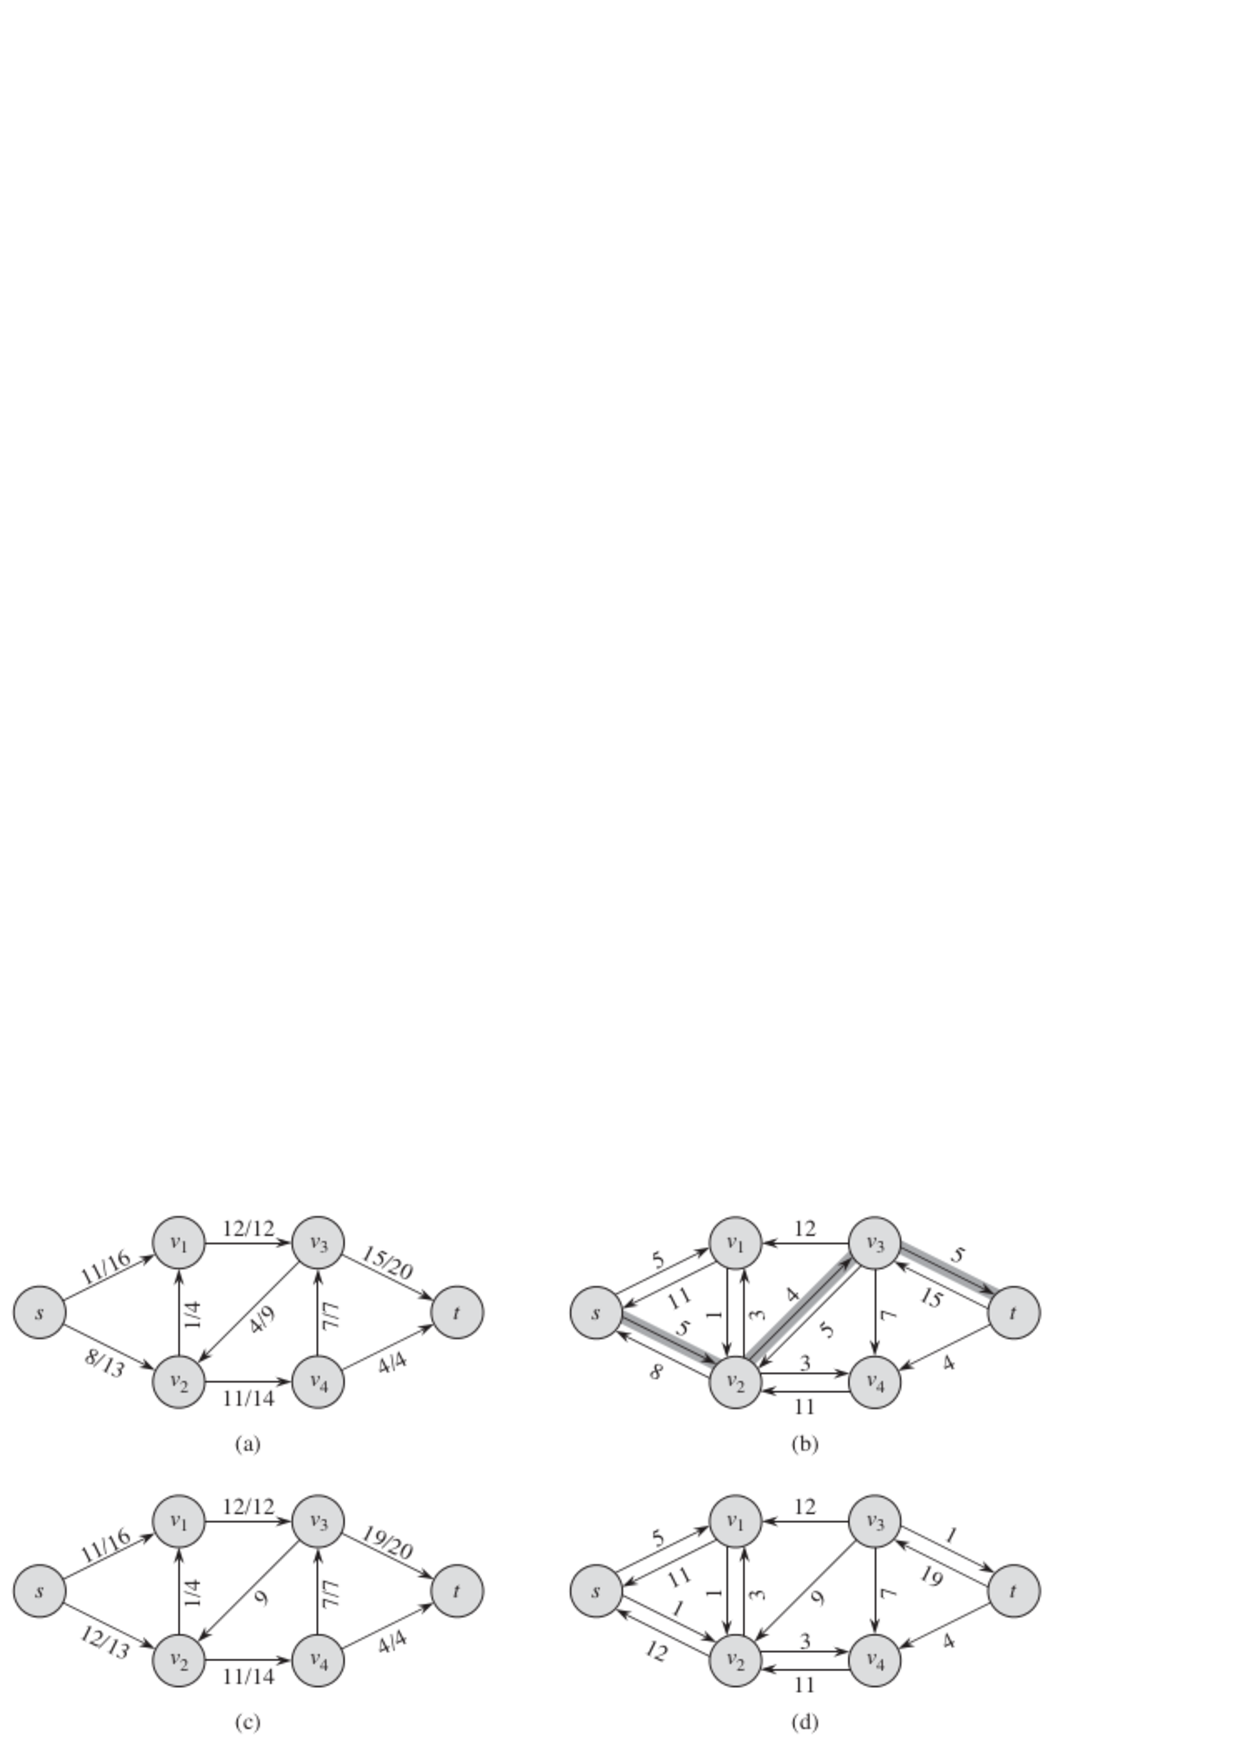
\includegraphics[width=\textwidth]{images/augmenting_paths}
\end{figure}
%%
Given a network $G = (V,E)$ with a flow $f$, the \textbf{residual network}
of $G$ induced by $f$ is $G_f = (V, E_f)$, where
%%
\[
	E_f = \{(u,v) \in V \times V : c_f(u,v) > 0\}.
\]
%%
Residual capacity $c_f(u,v)$ is defined by
%%
\[
 c_f(u,v) =
  \begin{cases}
  	c(u,v) - f(u,v) & \text{if } (u,v) \in E, \\
  	f(v,u) & \text{if } (v,u) \in E, \\
  	0 & \text{otherwise}
  \end{cases}
\]
%%
\textit{Note:} that $(u,v) \in E$ implies $(v,u) \notin E$, so there is always only one of the three
above cases that applies. 

Because the edges in $E_f$ are either edges from $E$ or an edge in the opposite direction,
$|E_f| \leq 2|E|$.

Intuition: A residual network $G_f$ consists of edges with capacities that
represent how we can alter the flow on edges of $G$. $G$ can admit an
additional amount of flow along an edge, equal to the capacity minus the
current flow. If the edge can admit more flow, that edge is placed into $G_f$
with a value of $c_f(u,v) = c(u,v) - f(u,v)$. The residual network may also
contain edges that are not in $G$: In order to represent a possible decrease
of a flow $f(u,v)$ on an edge in $G$, we place an edge $(v,u)$ into $G_f$ with
residual capacity $c_f(v,u) = f(u,v)$. In other words, an edge that can admit
flow in the opposite direction, at most cancelling out flow entirely. See
Figure~\ref{fig:aug_paths} for an example.

Flows in a residual network satisfy the definition of a flow, but with respect to capacities
$c_f$ in the network $G_f$. If $f$ is a flow in $G$ and $f'$ is a flow in the corresponding residual
network $G_f$, we define $f \uparrow f'$, the \textbf{augmentation flow} of f by f', as a function
from $V \times V$ to $\mathbb{R}$ defined by
%%
\[
  (f \uparrow f')(u,v) =
  \begin{cases}
  	f(u,v) + f'(u,v) - f'(v,u) & \text{if } (u,v) \in E, \\
  	0 & \text{otherwise.}
  \end{cases}
\]

Intuition: Increase the flow ($f(u,v)$) by $f'(u,v)$, but decrease it by the flow in the
opposite direction ($f'(v,u)$). Pushing flow in the reverse direction is also called \textbf{cancellation}.

\subsubsection{Augmenting path}
An augmenting path $p$ is a simple path from $s$ to $t$ in the residual network $G_f$. By the definition
of a residual network, we may increase the flow of an edge $(u,v)$ by up to $c_f(u,v)$ without violating the
capacity constraint on whichever of $(u,v)$ and $(v,u)$ is in the original flow network $G$.

The maximum amount by which we can increase flow on each edge of an augmenting path $p$ is the
\textbf{residual capacity} of $p$, given by $c_f(p) = min\{c_f(u,v) : (u,v) \text{ is on p}\}$. More specifically,
if $p$ is an augmenting path in $G_f$, we define a function $f_p : V \times V \rightarrow \mathbb{R}$ as
%%%
\[
	f_p(u,v) =
	\begin{cases}
		c_f(p) & \text{if } (u,v) \text{is on } p, \\
		0 & \text{otherwise}.
	\end{cases}
\]
%%
Then $f_p$ is a flow in $G_f$ with value $|f_p| = c_f(p) > 0$. See Lemma 26.2, page 720. It remains to be
shown that augmenting $f$ by $f_p$ produces a different flow in $G$ whose value is closer to the maximum.
Corollary 26.3 on page 720 shows this by immediate proof, using Lemma 26.1 and 26.2.
\newpage

\subsection{Fibonacci Heaps}
\todo[inline]{Write something about mergable heaps} Fibonacci heaps are a
datastructure that supports a set of operations qualifying it as a ``meargeable
heap'', meaning it supports the following operations.

\begin{itemize*}
  \item \texttt{Make-Heap()} Creates and returns a new heap with no elements.
  \item \texttt{Insert(H,x)} Inserts element $x$ whose key have already been
    filled in., into heap $H$.
  \item \texttt{Minimum(H)} Returns a pointer to the element in heap $H$ whose
    key is minimum.
  \item \texttt{Extract-Min(H)} Deletes the element from heap $H$ whose key is
    minimum, returning a pointer to the element.
  \item \texttt{Union(H$_1$,H$_2$)} Creates and returns a new heap that contains
    all the elements of both heaps. Both heaps are destroyed by the operation.
\end{itemize*}

Apart from the meargeable heap operations above, Fibonacci Heaps also support
the following two operations.

\begin{itemize*}
\item \texttt{Decrease-Key(H,x,k)} Assigns to element $x$ in heap $H$ the new
  key value $k$, which cannot be greater than it's current value.
  \item \texttt{Delete(H,x)} Deletes element $x$ from $H$.
\end{itemize*}

Fibonacci Heaps are by default min-heaps, but could just as well be max heaps,
then we would just replace the Minimum, Extract-Min and Decrease-Key operations
with Maximum, Extract-Max and Increase-Key instead.

Fibonacci Heaps have a benefit in the fact that many operations are run in
constat amortized time. So if these operations are used frequently, the
Fibonacci Heap is a well suited structure.

\begin{table}[h]
\begin{tabular}{lll}
  Procedure    & Binary heap(worst case) & Fibonacci heap (amortized) \\ \hline
  Make-heap    & $\Theta(1)$             & $\Theta(1)$ \\
  Insert       & $\Theta(lg n)$          & $\Theta(1)$ \\
  Minimum      & $\Theta(1)$             & $\Theta(1)$ \\
  Extract-Min  & $\Theta(lg n)$          & $O(lg n)$ \\
  Union        & $\Theta(n)$             & $\Theta(1)$ \\
  Decrease-Key & $\Theta(lg n)$          & $\Theta(1)$ \\
  Delete       & $\Theta(lg n)$          & $O(lg n)$
\end{tabular}
\caption{Amortized running times of normal binary heaps and Fibonacci Heaps.}
\end{table}

\subsubsection{Structure}

A Fibonaccci Heap is a collectoin of rooted trees that are ``min-heap
ordered''. That is, each tree obeys the minimum-heap property: The key of a node
is greater than or equal to the key of its parent. A node $x$ contains a pointer
$x.p$ to its parent and a pointer $x.child$ to any one of its children. This
list is called the child list. Each node also contains 2 pointers $x.left$ and
$x.right$, these points to a nodes siblings or to the node itself if it has n
osiblings. This forms a circular doubly-linked list called the child list. The
nodes may appear in the child list in any order.

Nodes have 2 additional properties, $x.degree$ which is how many children a node
have, and a boolean value $x.mark$. $x.mark$ indicates if $x$ has lost a child
since $x$ was made the child of another node. Nodes initially have $x.mark =$
False.

\graphicc{1}{img/fib_heaps_example}{An example of a Fibonacci Heap with(b) and
  without(a) the child-list.}{fig:figexample}

We access a fibonacci Heap by the pointer $H.min$ which points to the root of a
tree containing the minimum key, this node is called the minimum node. If there
are several nodes with the smallest key, any of those will work. When the heap
is empty, $H.min =$ NIL. The roots of all the tree in a Fibonacci Heap ar linked
togeter in a circular doubly-linked list called the ``root list''. $H.min$
points to a node in the root list. The heap also have one other property, $H.n$
which is the number of nodes currently in $H$.

\subsubsection{Operations}

\begin{description}
\item[Make-Heap] Simply creates a pointer $H.min =$ NIL; since there is no trees
  in $H$ at this point. This operation can be performed in $O(1)$ time.

\item[Insert] Insertion is done on constant time as well.
  \begin{codebox}
    \Procname{$\proc{Fib-Heap-Insert}(H,x)$}
    \li $x.degree \gets 1$
    \li $x.p \gets \const{nil}$
    \li $x.child \gets \const{nil}$
    \li $x.mark \gets \const{false}$
    \li \If $H.min == \const{false}$ \Do
    \li   Create a root list for $H$ containing just $x$.
    \li   $H.min = x$
    \li \Else insert $x$ into $H$'s root list
    \li   \If $x.key < H.min.key$ \Do
    \li     $H.min = x$
          \End
        \End
    \li $H.n = H.n + 1$

  \end{codebox}

\item[Minimum] Just follow the $H.min$ pointer and you're home safe.

\item[Extract-Min] This is the most complicated and expensive of the meargeable
  heap procedures, since it will be doing the work of actually consolidating the
  trees in the list. Most other procedures put of this work so that it can be
  done when using Extract-Min. This operation can be done in $O(\text{lg }n)$
  time.
  \begin{codebox}
    \Procname{$\proc{Fib-Heap-Extract-Min}(H)$}
    \li $z.min \gets H.min$
    \li \If $z \neq \const{nil}$ \Do
    \li   \For each child $x$ of $z$ \Do
    \li     add $x$ to the root list of $H$
    \li     $x.p \gets \const{nil}$ \End
    \li   remove $z$ from the root list of $H$
    \li   \If $z == z.right$ \Do
    \li     $H.min \gets \const{nil}$
    \li   \Else $H.min \gets z.right$
    \li     $\proc{Consolidate}(H)$ \End
    \li   $H.n = H.n - 1$ \End
    \li \Return $z$
  \end{codebox}

  Notice that $D(H.n)$ here will calculate the upper bound on the degree.
  \begin{codebox}
    \Procname{$\proc{Consolidate}(H)$}
    \li let $A[0..D(H.n)] $ be a new array
    \li \For $i \gets 0$ \To $D(H.n)$ \Do
    \li   $A[i] \gets \const{nil}$ \End
    \li \For each node $w$ in the root list of $H$ \Do
    \li   $x \gets w$
    \li   $d \gets x.degree$
    \li   \While $A[d] \neq \const{nil}$ \Do
    \li     $y \gets A[d]$ \Comment another node with the same degree as $x$
    \li     \If $x.key > y.key$ \Do
    \li       exchange $x$ with $y$ \End
    \li     $\proc{Fib-Heap-Link}(H,y,x)$
    \li     $A[d] \gets \const{nil}$
    \li     $d \gets d + 1$ \End
    \li   $A[d] \gets x$ \End
    \li $H.min \gets \const{nil}$
    \li \For $i \gets 0$ \To $D(H.n)$ \Do
    \li   \If $A[i] \neq \const{nil}$ \Do
    \li     \If $H.min == \const{nil}$ \Do
    \li       create a root list for $H$ containing just $A[i]$
    \li       $H.min \gets A[i]$
    \li     \Else insert $A[i]$ into $H$'s root list \Do
    \li       \If $A[i].key < H.min.key$ \Do
    \li         $H.min = A[i]$
  \end{codebox}

  \begin{codebox}
    \Procname{$\proc{Fib-Heap-Link}(H,y,x)$}
    \li remove $y$ from the root list of $H$
    \li make $y$ a child of $x$, incrementing $x.degree$
    \li $y.mark \gets \const{false}$
  \end{codebox}


\item[Union] Merging two fibonacci Heaps are done in constant:
  \begin{codebox}
    \Procname{$\proc{Fib-Heap-Union}(H_1,H_2)$}
    \li $H \gets \proc{Make-Fib-Heap}()$
    \li $H.min \gets H_1.min$
    \li Concatenate the root list oh $H_2$ with the root list of $H$.
    \li \If $(H_1.min == \const{nil})$ or ($H_2.min \neq \const{nil}$ and $H_2.min.key < H_1.min.key)$ \Do
    \li   $H.min \gets H_2.min$ \End
    \li $H.n \gets H_1.n + H_2.n$
    \li \Return $H$
  \end{codebox}

\item[DecreaseKey]
  We can decrease the key of any node using this method, it runs in $O(1)$ time.
  \begin{codebox}
    \Procname{$\proc{Fib-Heap-Decrease-Key}(H,x,k)$}
    \li \If $k > x.key$ \Do
    \li   \Error new key is greater than current key"\End
    \li $x.key \gets k$
    \li $y \gets x.p$
    \li \If $y \neq \const{nil}$ adn $x.key < y.key$ \Do
    \li   $\proc{Cut}(H,x,y)$
    \li   $\proc{Cascading-Cut}(H,y)$ \End
    \li \If $x.key < H.min.key$ \Do
    \li   $H.min \gets x$
  \end{codebox}
  \begin{codebox}
    \Procname{$\proc{Cut}(H,x,y)$}
    \li remove $x$ from the child list of $y$, decrementing $y.degree$
    \li add $x$ to the root list of $H$
    \li $x.p \gets \const{nil}$
    \li $x.mark \gets \const{false}$
  \end{codebox}
  \begin{codebox}
    \Procname{$\proc{Cascading-Cut}(H,y)$}
    \li $z \gets y.p$
    \li \If $z \neq \const{nil}$ \Do
    \li   \If $y.mark == \const{false}$ \Do
    \li     $y.mark \gets \const{true}$
    \li   \Else $\proc{Cut}(H,y,z)$
    \li     $\proc{Cascading-Cut}(H,z)$\End
  \end{codebox}


\item[Delete] Since it uses two previusly defined functions, the amortized
  runningtime is easily calculated to $O(\text{lg }n)$.
  \begin{codebox}
    \Procname{$\proc{Fib-Heap-Delete}(H,x)$}
    \li $\proc{Fib-Heap-Decrease-Key}(H,x,-\infty)$
    \li $\proc{Fib-Heap-Extract-Min}(H)$
  \end{codebox}
\end{description}

\todo[inline]{Wrwite something about $D(n)$ since it's used for all the proofs.}
\newpage

\subsection{NP-Completeness}
Example of a problem in the $P$ class is an Euler Tour(a path in a graph that
uses all edges exactly once, vertices can be visited multible times) of a graph,
it can be done in $O(E)$. An $NP$ class example that is very similar is a
Hamiltonian cycle. A Hamiltonian cycle is a path that visits all vertices once.

We have three classes of problems in this subject:
\begin{itemize*}
\item[\textbf{P}] Problems that are solvable in polynomial time ($O(n^k)$ for
  some constant $k$.)
\item[\textbf{NP}] Problems that are verifiable on polynomial time, i.e. if we
  have a certificate/solution, can we check it in polynomial time. All problems
  in P will also be in NP.
\item[\textbf{NPC}] A subclass of NPC problems that are ``at least as hard as
  the hardest problems in NP'', these cannot be verified in polynomial time.
\end{itemize*}

\subsubsection{Decision problems vs. optimization problems}
NP-completeness does not cover optimization problems, only decision problems. We
can however use the relationship between optimization and decision problems to
guage if a optimization problems is in fact NP-complete.

The shortest-path problem is an opimization problem, but can converted (in
polynomial time) to a decision problem if the question is posed like so: ``Does
a path $p$ in the graph $G$ exist with only $k$ edges?'', then we iterate over
$k$ and will be able to guage the shortest bath problem as a dicision problem.

\todo[inline]{Continue from p. 1051}

\newpage

\subsection{Randomized Algorithms}

When talking random variables there are generally 3 kinds:
\begin{enumerate*}
  \item Las Vegas algorithms
  \item Monte Carlo algorithms with one-sided error
  \item Monte Carlo algorithms with two-sided error
\end{enumerate*}

A Las Vegas algorithm is a randomized algorithm that have zero possibility of
producing an invalid solution but where the running time is affected vy the
randomization.

A Monte Carlo algorithm is a randomized algorithm that might produce an
incorrect solution. For decisions problems these can be one-sided or
two-sided. A one sided algorithm is always correct for one of the answer
(yes/no) but might be wrong on the other one. If it is two-sided then it might
be wrong on both answers.


\subsubsection{Markov \& Chebyshev's inequalities}
\begin{description}
\item[Markov inequality] Let $Y$ be a random variable assuming only non-negative
  values. Then for all $t \in \mathbb{R}^+$,
  \[
    \text{Pr}[Y \geq t] \leq \frac{\text{E[Y]}}{t}.
  \]
  Equivalently,
  \[
    \text{Pr}[Y \geq k\text{E}[Y]] \leq \frac{1}{k}.
  \]
\item[Proof] Define a function $f(y)$:
  \[
   f(y) = \begin{cases}
     1 & \text{iff } y \geq t\\
     0 & \text{otherwise.}
   \end{cases}
  \]
  Then $\text{Pr}[Y \geq t] = \text{E}[f(y)]$. Since $f(y) \leq y/t$ for all $y$,
  \[
    \text{E}[f(Y)] \leq \text{E}\left [\frac{Y}{t} \right ] = \frac{\text{E}[Y]}{t},
  \]
  and the theorem follows. \qed
\end{description}

\begin{description}
\item[Chebyshevs inequality] Let $X$ be a random variable with expectation
  $\mu_X$ and a standard deviation of $\sigma_X$. Then for any $t \in
  \mathbb{R}^+$,
  \[
    \text{Pr}[|X - \mu_X| \geq t\sigma_X] \leq \frac{1}{t^2}
  \]
\item[Proof] Note that
  \[
    \text{Pr}[|X - \mu_X| \geq t\sigma_X] = \text{Pr}[(X - \mu_X)^2 \geq
    t^2\sigma_X^2]
  \]
  The random variable $Y = (X - \mu_X)^2$ has expectation $\sigma_X^2$, and
  applying the Markov inequality to $Y$ bounds this probability from above by
  $1/t^2$. \qed
\end{description}

\todo[inline]{Write about lazy select or randomized quicksort}
\newpage

\subsection{Exact Exponential Algorithms \& Fixed-Parameter Tractable Problems}

\subsubsection{Exact Exponential Algorithms}
The $O^*$ notation is similar to the $O$ notation, except it will suppress
running-times of polynomial itme. This means that factors that are not
exponential are suppressed. For example $O(kn^kk^n) = O(n^kk^n)$ but we have
$O^*(kn^kk^n) = O^*(k^n)$.

\noindent \textbf{Size vs length:} When we talk about the running time we usually talk about
the time in relation to the input size of length. For instance: Given a graph, the input size
will be $O(V + E)$ while the length will be the number of bits it takes to encode the input with any reasonable encoding.

For the travelling salesman problem (er permutation problem) the input is a set of $n$ cities, where we want to find
the correct permutation. In this case candidate solutions are sets of $n$ cities, of which there is $n!$. Thus
the trivial algorithm runs in $O^*(n!)$.

\noindent \textbf{Travelling Salesman using Dynamic Programming} \\
For a subset of cities $S \subset \{1,2,...,n\}$ that includes $1$, and $j \in S$, let $C(S,j)$ be
the length of the shortest path visiting each node in $S$ exactly once, starting at $1$ and ending at $j$.
When $|S| > 1$, we define $C(S,1) = \infty$ since the path cannot start and end at $1$.

We can express $C(S,j)$ in smaller sub-problems. We start at $1$ and end at $j$; for the second to last
city we have to pick some $i \in S$, so the overall path length is the distance from $1$ to $i$; namely,
$C(S-\{j\},i)$ plus the length of the final edge $d_{ij}$. We pick the best such $i$:
\[
  C(S,j) = \underset{i\in S:i\neq j}{\text{min}} C(S-\{j\},i)+d_{ij}
\]
The sub problems will be ordered by $|S|$.

\begin{codebox}
\Procname{$\proc{ExactTSP}(\{c_1,c_2,...c_n\},d)$}
\li $C(\{1\},1) \gets 0$
\li \For $s \gets 2$ \To $n$ \Do
\li   \For all subsets $S \subset \{c_1,c_2,...c_n\}$ of sizes $s$ and containing $1$ \Do
\li     $C(S,1) \gets \infty$
\li     \For all $j \in S, j\neq 1$ \Do
\li       $C(S,j) = \text{min}\{C(S-\{j\},i) + d_{ij} : i \in S, i \neq j\}$ \End\End\End
\li \Return $\text{min}_jC(\{1,...,n\},j) + d_{j1}$
\end{codebox}

There are at most $2^nn$ sub-problems, and each one takes linear time giving a final running time of $O(n^22^n)$ or $O^*(2^n)$.

\graphicc{1}{img/exacttsp.png}{A run of the exact TSP algorithm}{fig:exacttspsample}


\subsubsection{Fixed-Parameter Tractable Problems}
Roughly speaking, parameterized complexity seeks the possibility of obtaining
algorithms whose running time can be bounded by a polynomial function of the
input length and, usually, an exponential function of a parameter which is independent of the input.

We strive to understand a problem and its sub-problems in terms of parameters and their effects on the
running time, ideally the goal is to be able to form statements such as ``If some parameter $k$ is
small in problem $X$ then $X$ can be solved efficiently''. For instance in the vertex cover problem, we know that the solution
should be as few vertices as possible, so if $k$ is the solution size the exponential factor of the running time is less than $1.28^k$.

\noindent\textbf{CNF satisfiability}\\
A CNF problem is a conjunction of $m$ clauses where each clause consists of a disjunction of literals.
There there be $n$ different variables occurring in the formulae.

\begin{description}
\item[Parameter ``Clause Size''] The maximum number of $k$ literals a clause
  may contain. For $k = 2$ (2-CNF satisfiability) the running time is polynomial
  time solvable, however for $k = 3$ (3-CNF satisfiability) is NP-Complete.

\item[Parameter ``Number of Variables''] The number $n$ of different variables
  allowed in the formula. Since there is essentially $2^n$ different truth
  assignments, the problem can be solved in that number of steps, seeing that
  the result of each assignment can be calculated in a number of steps equal to
  the Number of clauses.

\item[Parameter ``Number of Clauses''] If the number of clauses in a formulae is
  bounded from above by $m$, the CNF problem can be solved in $1.24^m$ steps.

\item[Parameter ``Formula Length''] If the total length (counting the number of
  literal occurrences in the formula) of the formula $F$ is bounded by above by
  $\ell = |F|$, then the problem can be solved in $1.08^\ell$ steps.
\end{description}


\noindent \textbf{Maximum CNF Satisfiability}\\
An optimization version of the above problem. Here we want to satisfy as many clauses as possible and
not just the entire formulae. This problem shares the same parameters, but gives different effects.

\begin{description}
\item[Parameter ``Clause Size''] Even for $k = 2$ the problem is still NP-Complete.

\item[Parameter ``Number of Variables''] Like the decision problem, this one can be solved in $2^n$
  steps, where $n$ is the number of variables in the formulae. For $k=3$ it is still an open problem to obtain a better bound.
  Recently advances were made for $k=2$ allowing it to be solved in $1.74^n$ steps.

\item[Parameter ``Number of Clauses''] IFw e can bound the number of clauses above by $m$, the Maximum
Satisfiability problem can be solved in $1.33^m$ steps, and the Maximum 2 Satisfiability problem can be solved in $1.15^m$ steps.

\item[Parameter ``Formula Length''] If the total length (counting the number of
  literal occurrences in the formula) of the formula $F$ is bounded by above by
  $\ell$, Maximum Satisfiability problem can be solved in $1.11^\ell$ steps, and the Maximum 2 Satisfiability problem can be solved in $1.08^\ell$ steps.
\end{description}


\todo[inline]{VRÆÆÆÆÆÆÆÆLLLLL :(}
\newpage

\section{Approximation Algorithms: Disposition}
\begin{enumerate}
	\item Performance ratio
	\item Vertex-cover
	\item Traveling-salesman
	\item Set-covering
	\item Randomization \& Linear programming
	\item Subset-sum problem
\end{enumerate}

CLRS 35.1, 35.2, 35.3, 35.4, 35.5

\section{Approximation Algorithms: Notes}
An approximation algorithm is an algorithm that computes a near-optimal solution,
often because the optimal solution is NP-complete and thus intractable or at least
exponential in running time. One solution to that is to only work on small problem sets,
where exponential time is fine. Another is to compute a near-optimal solution using an
approximation algorithm.

\subsection{Performance ratio}
We say that an algorithm for a problem has an \textbf{approximation ratio} of
$p(n)$ if, for any input of size $n$, the cost $C$ of the solution produced by
the algorithm is within a factor of $p(n)$ of the cost $C^*$ of an optimal
solution:
%
\[
	max\left( \frac{C}{C^*}, \frac{C^*}{C}\right) \leq p(n)
\]
%
If an algorithm achieves an approximation ratio of $p(n)$ we call it a
$p(n)$\textbf{-approximation algorithm}. Because we assume all solutions have
a positive cost, these ratios are always well-defined. The approximation ratio of
an approximation algorithm is never less than 1, since $C/C^*\leq 1$ implies $C^*/C \geq 1$.
Therefore, a 1-approximation algorithm produces an optimal solution, and an approximation
algorithm with a large approximation ratio may return a solution much worse than optimal.

Below some schemes are outlined which allow us to give a value $\epsilon$ along
with the instance of the problem and achieve an approximation that have a
quality depending on the value.
\begin{description}
\item[Approximation Scheme] for an optimization problem is an approximation
  algorithm that takes as input, not only an instance of the problem, but also a
  value $\epsilon > 0$ such that for any fied $\epsilon$ the scheme is a
  $(1+\epsilon)$-approximation algorithm.

\item[Polynomial-Time Approximation Scheme] is an approximation scheme if for
  any fixed $\epsilon > 0$, the scheme runs in polynomia ltime in the size $n$
  of it's input instance. The running time of such a scheme can increase rapidly
  as $\epsilon$ decreases. For example, the running time of a polynomial-time
  approximation scheme might be $O(n^{(2/\epsilon)})$. Ideally, if $\epsilon$
  decrease by a constant factor, the running time to achieve the desired
  approximation should not incrase by more than a constant factor. (Not
  necessarily by the same factor $\epsilon$ was decreased with.)

\item[Fully Polynomial-Time Approximation Scheme] means the approximation
  algorithm runs in polynomial time in both $1/\epsilon$ and the size $n$ of the
  input instance. I.e. $O((1/\epsilon)^2n^3)$. With such a scheme, a constant
  factor decrease in $\epsilon$ comes with a constant factor increase in
  runningtime.
\end{description}

\subsection{Vertex-cover}
A Vertex Cover of an undirected graph $G = (V,E)$ is a subset $V' \subseteq V$
such that if $(u,v)$is an edge of $G$, then either $u \in V'$ or $v \in V'$ or
both. The size of a vertex cover is the number of vertices in it.

The Vertex Cover Problem is to find a vertex cover of minimum size in a given
undirected graph, this is an optimization version of an NP-Complete decision
problem.

\begin{description}
\item[Theorem 35.1] \texttt{Approx-Vertex-Cover} is a polynomial-time
  2-approximation algorithm.
\item[Proof] It is already shown that the algorithm is a polynomial time
  algorithm.

  The set $C$ of vertices return must be a vertex cover since it loops until
  every edge in $G.E$ have been covered by some vertex.

  To see that the algorithm returns a vertex cover of at most twice the size of
  an optimal cover, let $A$ denote the set og edges that line 4 selects.  To
  cover all the edges in $A$, any vertex cover, in particular the optimal vertex
  cover $C^*$, must include at least one endpoint of each edge in $A$. No two
  edges share endpoints since when an edge is picked, all edges incident on its
  endpoints are removed. Thus no two edges in $A$ are covered by the same vertex
  from $C^*$, and we have the lower bound
  \[
    |C^*| \geq |A|
  \]
  on the size of an optimal vertex cover. Each execution of line 4 picks an edge
  which neither of its endpoints are already in $C$, yielding an upper boind on
  the size of the vertex cover returned
  \[
    |C| = 2|A|
  \]
  Combining the two bounds gives
  \begin{align*}
    |C| &= 2|A| \\
        &\leq 2|C*|
  \end{align*}
  thereby proving the theorem. \qed
\end{description}

\subsection{Travelling-salesman}
The TSP is also NP-Complete, the following is a method for approximating an
optimal solution that is at most twice as long as the optimal tour.

It creates a minimum spanning tree using Prims algorithm, and walks along this
tree using a pre-order walk (parent first then child), and uses this as the
solution.

\begin{description}
\item[Theorem 35.2] \texttt{Approx-TSP-Tour} is a polynomial-time
  2-approximation algorithm for the traveling salesman problem, with the
  triangle inequality.

\item[Proof] See page 1114.
\end{description}

\subsection{Set-covering}
\subsection{Randomization \& Linear programming}
\subsection{Subset-sum problem}
\newpage

\subsection{Computational Geometry}
Let $P = \{p_1, p_2, ..., p_n\}$ be a set of points in the plane. To be able to
properly define the triangulation of the plane we first define the ``maximal
planar subdivision'' as a subdivision $\mathcal{S}$ such that no edges that
connects two vertices can be added without destroying the planarity.

A triangulation of $P$ is now defined as a maximal planar subdivision whose
vertex set is $P$.

\begin{description}
\item[Theorem] Let $P$ be a set of $n$ points in the plane, not all collinear,
  and let $k$ denote the number of points in $P$ that lie on the boundary of the
  convex hull of $P$. Then any triangulation of $P$ has $2n−2−k$ triangles and
  $3n−3−k$ edges.

\item[Proof] Let $\mathcal{T}$ be a triangulation of $P$, and let $m$ denote the
  number of triangles of $\mathcal{T}$.  Note that the number of faces of the
  triangulation, which we denote by $n_f$, is $m+1$. Every triangle has three
  edges, and the unbounded face has $k$ edges.  Furthermore, every edge is
  incident to exactly two faces. Hence the total number of edges of
  $\mathcal{T}$ is $n_e = (3m+k)/2$. Euler's formula tells us that
  \[
    n-n_e+n_f = 2
  \]
  Plugging the values for $n_e$ and $n_f$ into the formula, we get $m=2n-2-k$,
  which in turn implies $n_e = 3n-3-k$. \qed
\end{description}


Let $\mathcal{T}$ be a triangulation of $P$, and suppose it has $m$
triangles. Consider the $3m$ angles of $\mathcal{T}$, sorted by increasing
value.  Let $\alpha_1, \alpha_2, ..., \alpha_{3m}$ be the resulting sequence of
angles. We call $A(\mathcal{T}) = (\alpha_1, \alpha_2, ..., \alpha_{3m})$ the
angle vector of $\mathcal{T}$.  Let $\mathcal{T}'$ be another triangulation of
the same point set $P$. We say that $A(\mathcal{T}) > A(\mathcal{T}')$ if
$A(\mathcal{T})$ if there exists and index $i$ with $1 \leq i \leq 3m$ such that
\[
\alpha_j = \alpha_j' \text{ for all } j < i, \text{\quad and \quad} \alpha_i >
\alpha_i'
\]
A triangulation $\mathcal{T}$ is called angle-optimal if $A(\mathcal{T}) \geq
A(\mathcal{T}')$ for all triangulations $\mathcal{T}'$ of $P$.  These are good
because slender triangles make for bad triangulations for terrain.

\textit{Denote the smaller angle defined by three points $p,q,r,$ as
  $\measuredangle pqr$.}

\begin{description}
\item[Thales Theorem] Let $C$be a circle, $\ell$ be a line intersecting $C$ in
  points $a$ and $b$. Let $p, q, r$ and $s$ be points lying on the same side fo
  $\ell$. Suppose that $p$ and $q$ lie on $C$, that $r$ lies inside $C$ nad that
  $s$ lies outside $C$.  Then
  \[
    \measuredangle arb > \measuredangle apb = \measuredangle aqb > \measuredangle asb.
  \]
  \graphicc{0.4}{img/compgeo0.png}{The circle $C$ and the points drwan for
    clarity.}{fig:compgeo0}

\item[Illegal edge] Consider an edge $e = \overline{p_ip_j}$ of a triangulation
  $\mathcal{T}$. If $e$ is not on the unbounded face, it is incident on two
  triangles, $p_ip_jp_k$ and $p_ip_jp_l$. If these triangles form a convex
  quadrilateral, we can obtain a new triangulation $\mathcal{T}'$ by flipping
  the edge. This is done by removing $\overline{p_ip_j}$ and adding
  $\overline{p_kp_l}$. This changes the anglevectors, but only the entries
  associated with the two triangles.  An edgeis considered illegal if flipping
  it increase $A(\mathcal{T})$ such that
  \[
    \underset{1\leq i \leq 6}{\min} \alpha_i < \underset{1\leq i\leq 6}{\min} \alpha_i'.
  \]
  An edge is illegal if we can locally increase the smallest angle simply by flipping it.

\item[Observation 9.3] Let $\mathcal{T}$ be a triangulation with an illegal edge
  $e$. Let $\mathcal{T}'$ be the triangulation obtained from $\mathcal{T}$ by
  flipping $e$. Then $A(\mathcal{T}) > A(\mathcal{T}')$.

\item[Lemma 9.4] Let edge $\overline{p_ip_j}$ be incident on to triangles
  $p_ip_jp_k$ and $p_ip_jp_k$, and let $C$ be the circle through $p_i$, $p_j$
  and $p_k$. The dege $\overline{p_ip_j}$ is illegal iff. the point $p_l$ lies
  in the interior of $C$.  Furthermore, if the points $p_i, p_j, p_k$ and $p_l$
  form a convex quadrilateral and do not lie on a common circle, then exactly on
  of $\overline{p_ip_j}$ and $\overline{p_kp_l}$ is an illegal edge.
  \graphicc{0.4}{img/compgeo1.png}{Visualization of Lemma 9.4.}{fig:compgeo1}

\item[Legal Triangulation] A legal triangulation is simple a triangulation that
  contain no illegal edges. We note that any legal triangulation must also be an
  angle-optimal triangulation. Computing a legal triangulation is simple given
  any triangulation.  simply flip illegal edges until non remain. This is very
  slow though.
\end{description}



\subsubsection{Delaunay Triangulation}

\begin{codebox}
\Procname{$\proc{DelaunayTriangulation}(P)$}
\li Let $p_0$ be the lexicographically higest point og $P$ (largest $x$ and $y$ coordinate.)
\li Let $p_{-1}$ and $p_{-2}$ be two points in $\mathbb{R}^2$ sufficiently far away such \\
    that $P$ is contained in the triangle $p_0p_{-1}p_{-2}$
\li Initialize $\mathcal{T}$ as the triangulation consisting of $p_0p_{-1}p_{-2}$.
\li Compute a random permutation $p_1,p_2,...,p_n$ of $P$\textbackslash$\{p_0\}$.
\li \For $r \gets 1$ \To $n$ \Do
\li   \Comment{Insert $p_r$ into $\mathcal{T}$}
\li   Find a triangle $p_ip_jp_k \in \mathcal{T}$ containing $p_r$
\li   \If $p_r$ lies on the interior of the triangle \Do
\li     Add edges from $p_r$ to the three vertices $p_ip_jp_k$, splitting it into three triangles.
\li     $\proc{LegalizeEdge}(p_r, \overline{p_ip_j}, \mathcal{T})$
\li     $\proc{LegalizeEdge}(p_r, \overline{p_jp_k}, \mathcal{T})$
\li     $\proc{LegalizeEdge}(p_r, \overline{p_kp_i}, \mathcal{T})$
\li   \Else \Comment{$p_r$ must lie on an edge, say $\overline{p_ip_j}$}
\li     Add edges from $p_r$ to $p_k$ and to the third vertex $p_l$ of the other triangles that is \\
        incident to $\overline{p_ip_j}$, thereby splitting the two triangles incident to \\
        $\overline{p_ip_j}$ into four triangles.
\li     $\proc{LegalizeEdge}(p_r, \overline{p_ip_l}, \mathcal{T})$
\li     $\proc{LegalizeEdge}(p_r, \overline{p_lp_j}, \mathcal{T})$
\li     $\proc{LegalizeEdge}(p_r, \overline{p_jp_k}, \mathcal{T})$
\li     $\proc{LegalizeEdge}(p_r, \overline{p_kp_i}, \mathcal{T})$ \End \End
\li Discard  $p_{-1}$ and $p_{-2}$ and all their incident edges from $\mathcal{T}$.
\li \Return $\mathcal{T}$
\end{codebox}

\begin{codebox}
\Procname{$\proc{LegalizeEdge}(p_r, \overline{p_ip_j}, \mathcal{T})$}
\li \If $\overline{p_ip_j}$ is illegal \Do
\li   Let $p_ip_jp_k$ be the truangle adjacent to $p_rp_ip_j$ along $\overline{p_ip_j}$.
\li   Replace $\overline{p_ip_j}$ with $\overline{p_rp_k}$.
\li   $\proc{LegalizeEdge}(p_r, \overline{p_ip_k}, \mathcal{T})$
\li   $\proc{LegalizeEdge}(p_r, \overline{p_kp_j}, \mathcal{T})$
\end{codebox}

\graphicc{0.8}{img/compgeo2.png}{An example insertion of $p_r$ and a calls to
  legalize edge.}{fig:compgeo2}


\begin{description}
\item[Lemma 9.10] Every new edge created in \texttt{DelaunayTriangulation} or in
  \texttt{LegalizeEdge} during the insertion of $p_r$, is an edge of the
  Delaunay graph of $\{p_{-2},p_{-1},p_0,...,p_r\}$

\item[Proof] Consider first the edges $\overline{p_rp_i}$,
  $\overline{p_rp_j}$,$\overline{p_rp_k}$ (and perhaps $\overline{p_rp_l}$)
  created by splitting $p_ip_jp_k$ (and maybe $p_ip_jp_l$).  Since $p_ip_jp_k$
  is a triangle in the Delaunay triangulation before the addition of $p_r$, the
  circumcirle $C$ of $p_ip_jp_k$ contains no point $p_t$ with $t<r$ in its
  interior.  By shrinking $C$ we can find a circle $C'$ through $p_i$ and $p_r$
  contained in $C$.  Because $C' \subset C$ we know that $C'$ is empty. This
  implies that $\overline{p_rp_i}$ is an edge of the Delaunay graph after the
  addition of $p_r$. The same holds for $\overline{p_rp_j}$ and
  $\overline{p_rp_k}$ (and $\overline{p_rp_l}$ if it exists).

Now consider and edge flipped by \texttt{LegalizeEdge}. Such an edge flip always
replaces an edge $\overline{p_ip_j}$ of a triangle $p_ip_jp_l$ by and edge
$\overline{p_rp_l}$ incident to $p_r$.  Since $p_ip_jp_l$ was a Delaunay
triangle before the addition of $p_r$ and becauseits circumcircle $C$ contains
$p_r$ -- otherwise $\overline{p_ip_j}$ would not be illegal -- we can shrink the
circumcircle to obtain an empty circle $C'$ with only $p_r$ and $p_l$ on its
boundary. Hence $\overline{p_rp_l}$ is an edge of the Delaunay graph after the
addition \qed

\graphicc{0.4}{img/compgeo3.png}{Helpfull illustration for the proof. :)}{fig:compgeo3}

\end{description}

\todo[inline]{Look op the stuff on p. 202 of the comp geo paper, it's prett smart with pointers and trees.}
\newpage




\end{document}
